\section{2.3 Разработка}
\label{cha:development}

\subsection{2.3.1 Система тестирования}
Конечный продукт должен представлять собой сервис, который позволяет протестировать реализацию пространственных структур с соответствующими операциями под нагрузкой, а также сами алгоритмы, как взятые готовые решения, так и решения, разработанные в ходе данной работы. 
\begin{enumerate}
    \item Для реализации структур и алгоритмов был выбран язык программирования Golang.  
    \item Для клиентского взаимодействия с сервисом используется HTML и JavaScript.
    \item Для визуализации результатов тестирований используется библиотека ChartsJS.
    \item Для визуализации работы алгоритмов используется библиотека Mapbox.
\end{enumerate}
  \\
\begin{figure}[h]
    \centering
    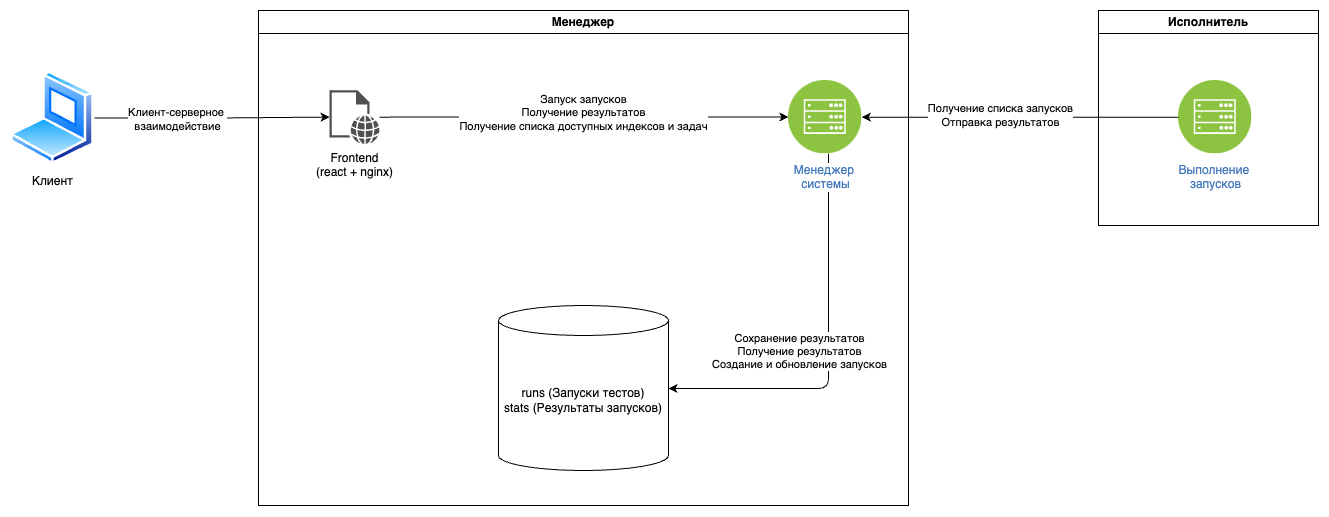
\includegraphics[scale=0.3]{arch.png}
    \caption{Архитектура системы тестирования}
\end{figure}
  \\
На рисунке 8 визуализирована архитектура решения. Компонент менеджер отвечает за управление и запуск тестов. Компонент \textit{Исполнитель} находится на отдельном от компонента \textit{менеджер} сервере и отвечает за запуск конкретных задач. Сделано это для того, чтобы как можно сильнее изолировать среду запуска и среду анализа и не влиять на результаты запуска тестов какими-либо другими задачами. 


\subsection{2.3.2 Порядок работы с программным обеспечением}
  \\
\begin{figure}[h]
    \centering
    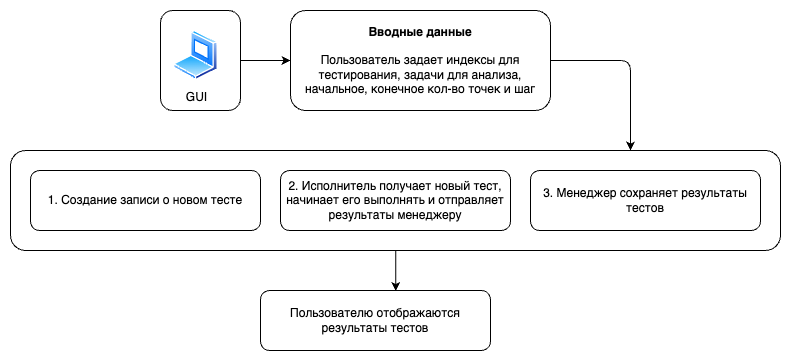
\includegraphics[scale=0.5]{seq.png}
    \caption{Функциональная схема}
\end{figure}
  \\
Процесс использования системы показан на рисунке 9: При открытии страницы с тестами (рисунок 10), пользователь может ознакомиться с доступными индексами и задачами, а также задать количество точек для тестирования. После нажатия кнопки «Старт» начнется тестирование, которое сразу создаст запись с тестом и результатами в виде графиков. 
Пользователь по своему усмотрению может остановить тестирование. Например, если оно выполняется слишком долго. Также он может открыть график с результатами в полном экране, а также скачать его. 
Также имеется страница «Визуализация данных» (рисунок 11), она может быть полезна для разработчиков во время разработки самих индексов, а именно для отладки индексов, визуализации их работы и сравнения с другими индексами. 

\begin{figure}[h]
    \centering
    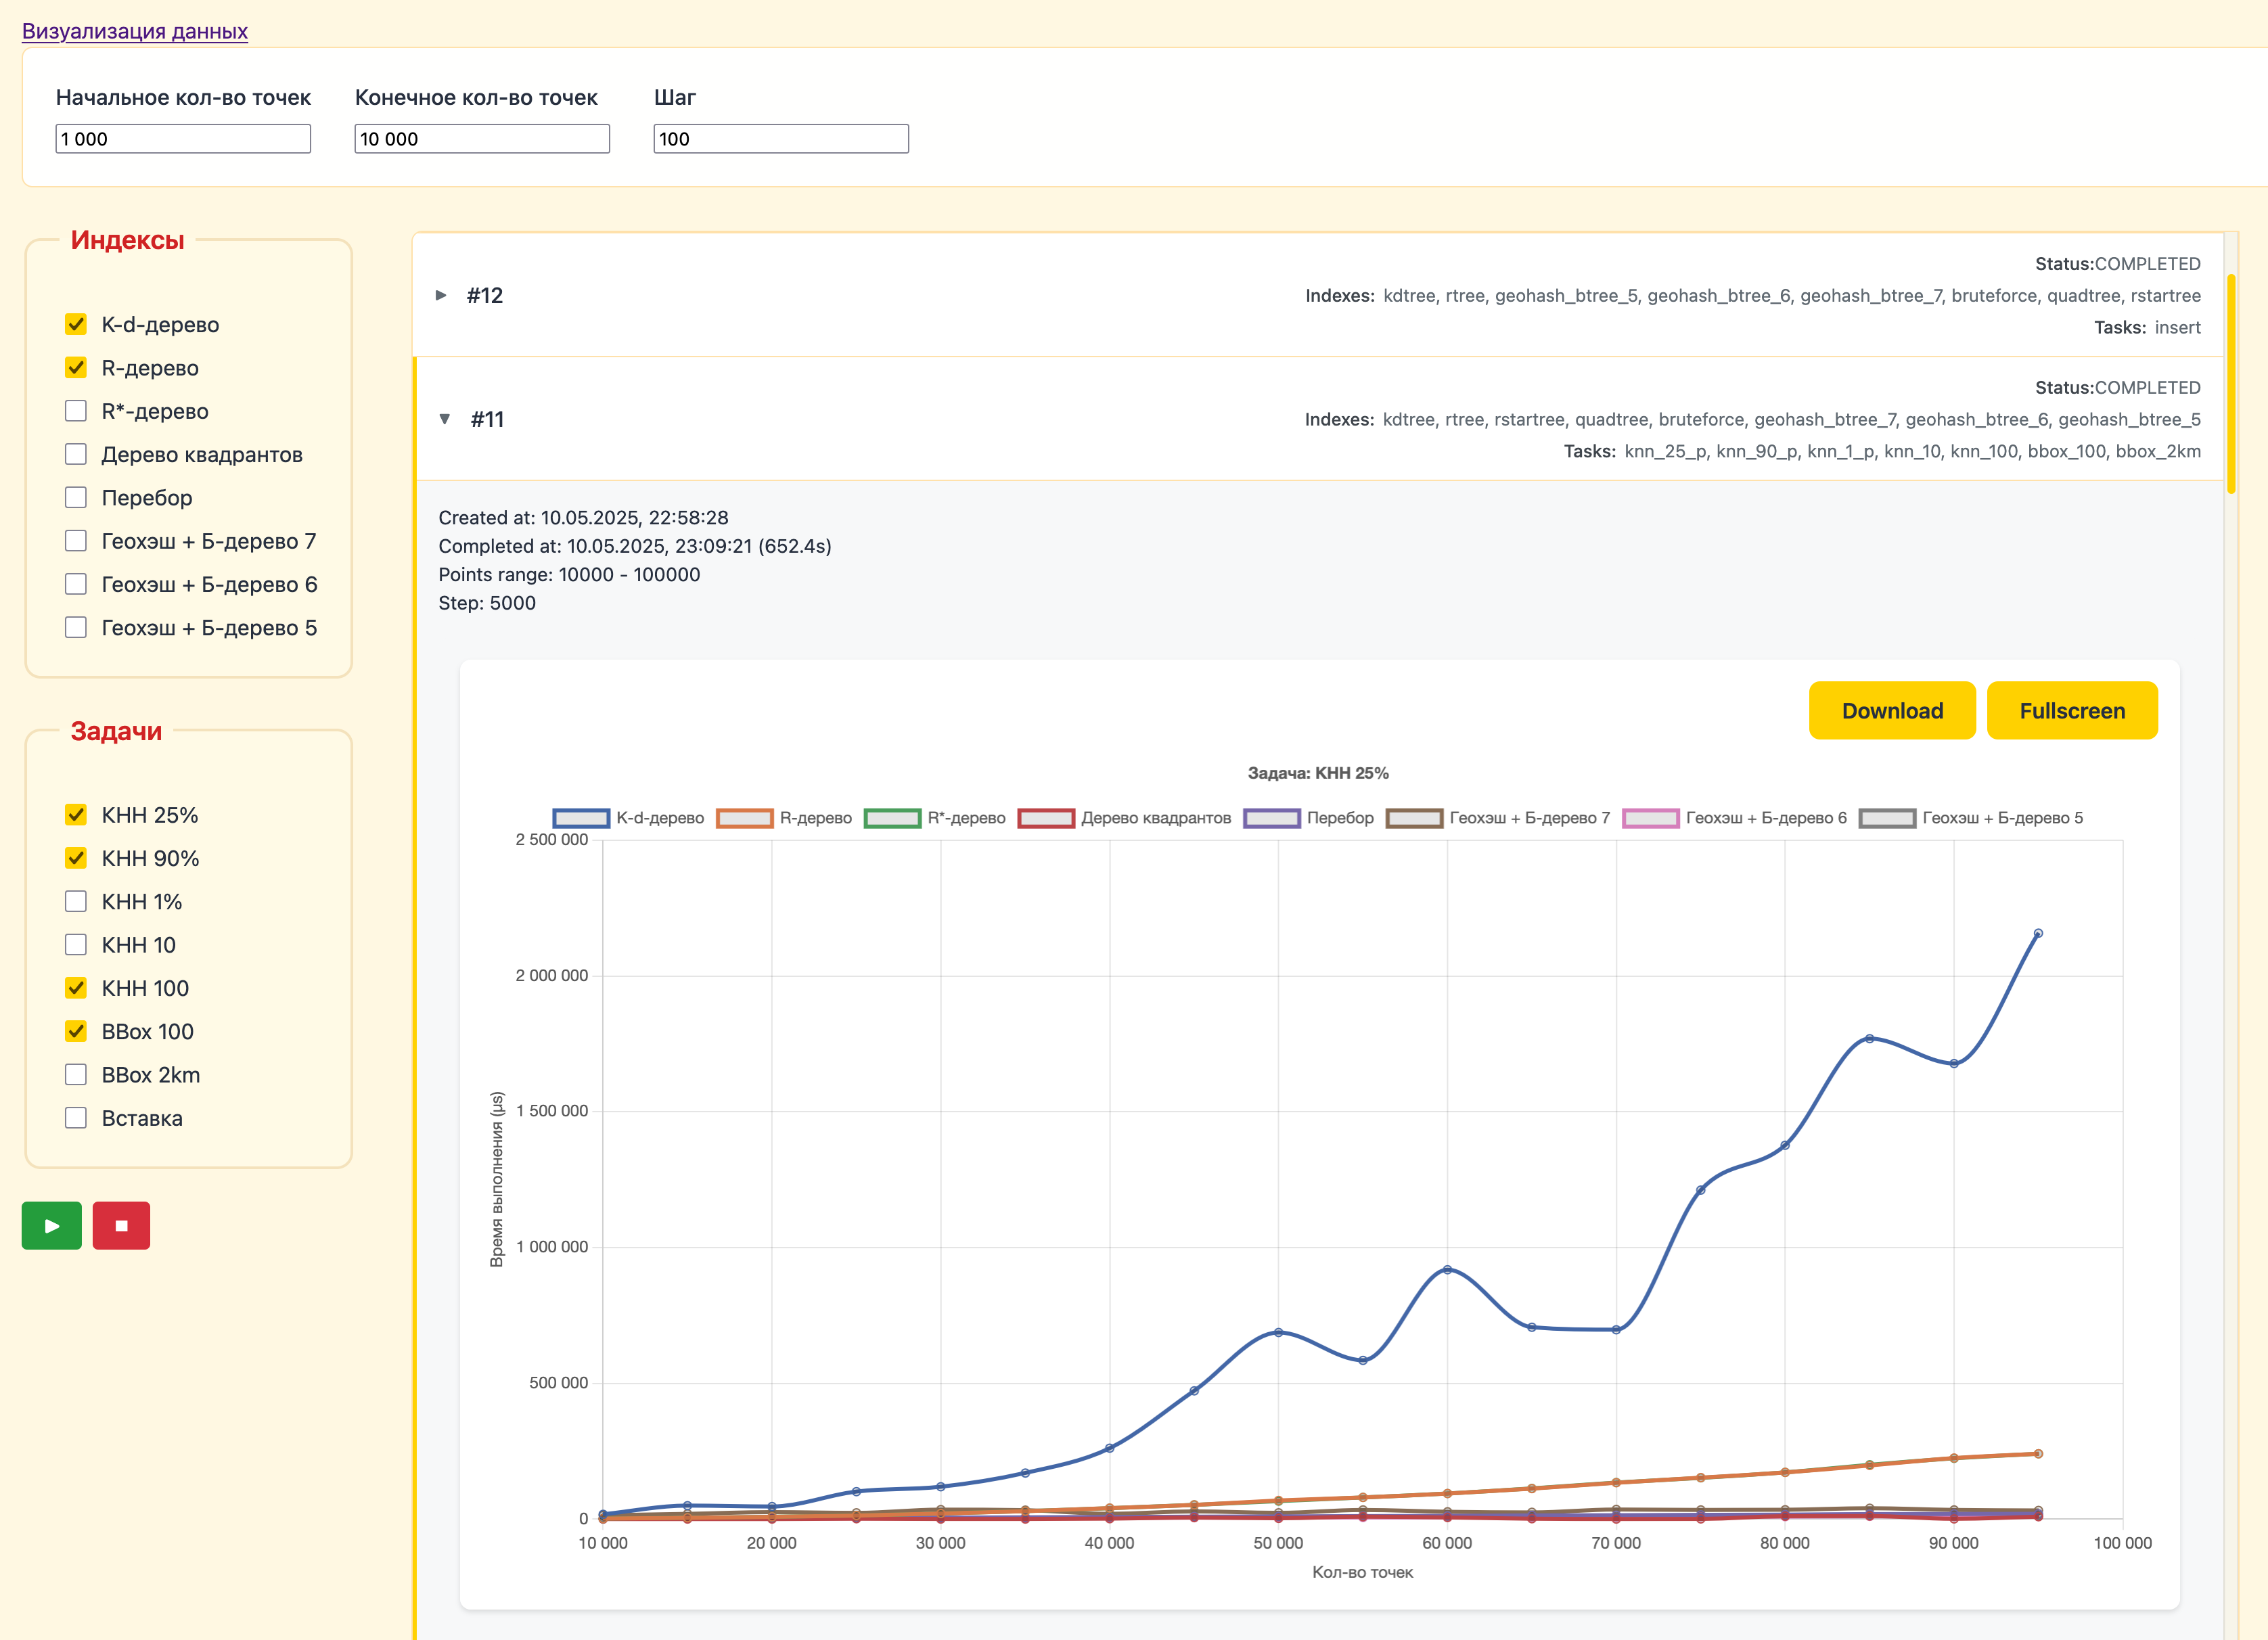
\includegraphics[scale=0.19]{gui.png}
    \caption{Главный экран}
\end{figure}

\begin{figure}[h]
    \centering
    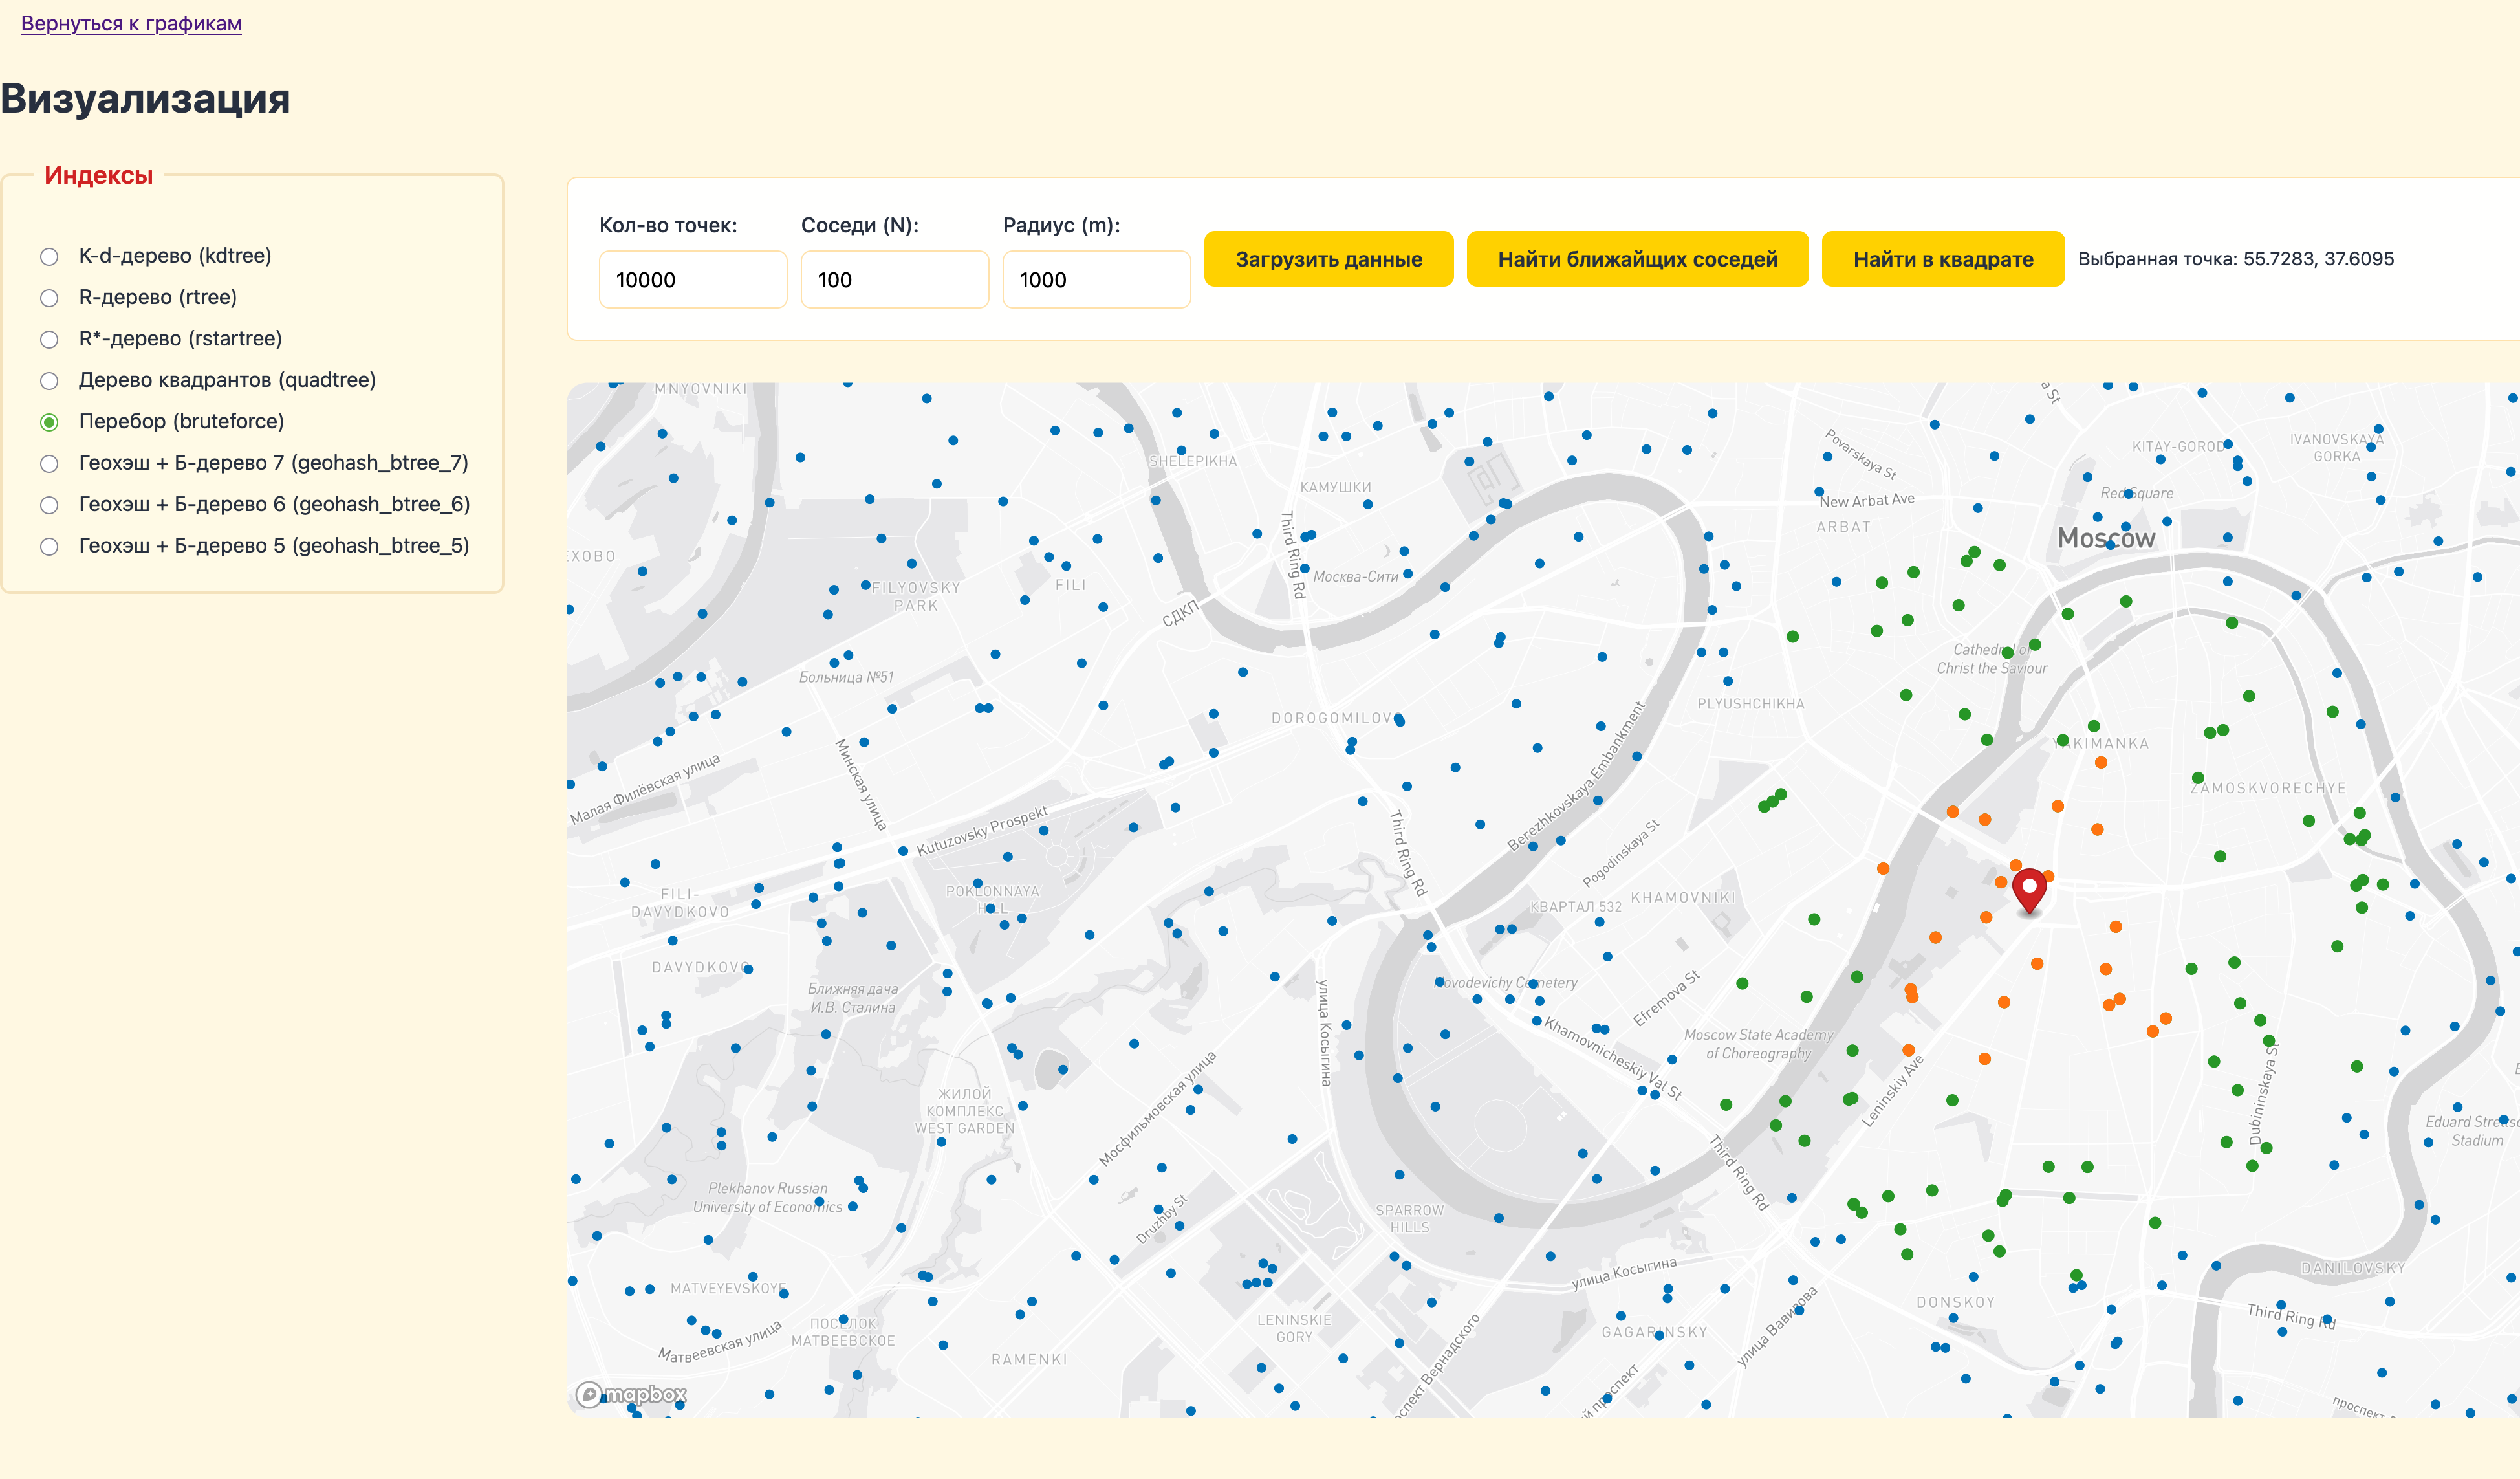
\includegraphics[scale=0.17]{gui_visualizer.png}
    \caption{Экран визуализации}
\end{figure}

С подробными результатами тестов можно ознакомится в приложение Б.